\testCom
{%Номер задачи
	3.150
}
{%Условие
	условие
}
{%Дано
	дано
}
{%Найти
	найти
}
{%Решение
	$\assume U = U_m \cos \omega t$\\
	а) $I_m \abs{Z} = U_m \Rightarrow I_m = \frac{U_m}{\abs{Z}}$, где\\
	$\abs{Z} = \sqrt{R^2 + (\frac{1}{\omega C } - \omega L)^2}$\\
	б) Запишем закон Ома для переменного тока:
	$I_m e^{\cancel{i \omega t} + \alpha} (R + i(\omega L - \frac{1}{\omega C})) = U_m \cancel e^{i \omega t}$\\
	$e^{i \alpha} \abs{Z} e^{i \psi} = \left( \frac{I_m}{U_m}\right)^{-1} e^0$\\
	$\alpha = - \psi = - \arctg \frac{\omega^2 L C - 1}{\omega C R}$\\\\
	в) $U_c = \abs{I \cdot X_C} = \abs{I} \cdot \abs{X_C} = I_m \cdot \frac{1}{\omega C}$\\
	$U_L = \abs{I \cdot R_L} = \abs{I} \abs{R + i \omega L} = I_m \sqrt{R^2 + L^2 \omega^2}$\\
	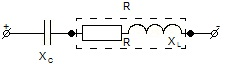
\includegraphics[height=30mm]{3_150.jpg}\\
}

